\documentclass[slovak]{scrartcl}
\usepackage[T1]{fontenc}
\usepackage[utf8]{inputenc}
\usepackage[usenames,dvipsnames]{pstricks}
\usepackage{epsfig}
\usepackage{pst-grad} % For gradients
\usepackage{pst-plot} % For axes
\usepackage{amsmath}

%opening
\title{Domáca úloha 1}
\subtitle{Dôkaz rovnice pre refrakciu lúča}
\author{Marek Kružliak}
\addtocounter{equation}{5}

\begin{document}

\maketitle

\section{Použité vzťahy a vlastnosti}

(1) Snellov zákon: $\eta_{1} \sin\theta_{1} = \eta_{2} \sin\theta_{2}$\\
(2) Veta pre sínus a cosínus: $\cos^{2}\theta + \sin^{2}\theta = 1$\\
(3) Uhol medzi dvoma vektormi: $ \cos\theta = \frac{\bar{u}\cdot\bar{v}}{|\bar{u}|\cdot|\bar{v}|}$\\
(4) Vektory vystupujúce v rovnici sú jednotkové: $|\bar{n}| = |\bar{\omega}| = |\bar{\omega}_{r}| = 1$\\ 
(5) Uhly $\theta_{1}$ a $\theta_{2}$ sú v intervale $<0,90>^{\circ} $\\
\\
Na tieto vzťahy sa budeme odkazovať neskôr v texte. \\
Lom lúča je znázornený na obrázku 1 na strane 3.

\section{Dôkaz}

Výsledný vektor $\bar{\omega}_{r}$ sa pokúsime získať skladaním dvoch vektorov $\bar{u}$ a $\bar{v}$: \\
\begin{equation} \bar{\omega}_{r} = \bar{u} +  \bar{v} \end{equation}
\\
Vektor $\bar{u}$ môžeme získať aj takto:
\begin{equation} \bar{u} = -\cos\theta_{2}\bar{n} \end{equation}
Kde $\cos\theta_{2} = \frac{|\bar{u}|}{|\bar{\omega_{r}}|} = |\bar{u}|$, keďže platí (4) a $-\bar{n}$ nám určuje smer vektora $\bar{u}$. Vektor $\bar{n}$ už poznáme a preto nám stačí dopočítať už len $\cos\theta_{2}$.\\
\\
Z (2) a (5) vieme, že: \begin{equation} \cos\theta_{2} = \sqrt{1 - \sin^{2}\theta_{2}} \end{equation}
Ďalej nám teda stačí vypočítať $\sin\theta_{2}$, na čo nám poslúži Snellov zákon.
\[ \sin\theta_{2} = \frac{\eta_{1}}{\eta_{2}}\cdot\sin\theta_{1}  \]
Na základe (2) a (5):
\begin{equation} \sin\theta_{2} = \frac{\eta_{1}}{\eta_{2}}\cdot\sqrt{1 - \cos^2\theta_{1}}  \end{equation}
Z (3) vieme vypoočítať $\cos\theta_{1}$:
\[ \cos\theta_{1} =   \frac{\bar{\omega}\cdot\bar{n}}{|\bar{\omega}|\cdot|\bar{n}|}\]
A keďže platí (4):
\begin{equation} \cos\theta_{1} = \bar{\omega}\cdot\bar{n} \end{equation}
Po doplnení $\cos\theta_{1}$ do (9), $\sin\theta_{2}$ do (8) a $\cos\theta_{2}$ do (7) získame vektor $\bar{u}$ takto:
\begin{equation}
 \bar{u} = -\left(\sqrt{1 - \left(\frac{\eta_{1}}{\eta_{2}}\right)^{2}(1 - (\bar{\omega}\cdot\bar{n})^2 )}\right)\bar{n}
\end{equation}
Teraz nám už en stačí získať vektor $\bar{v}$.\\
Vďaka (4) vieme, že $\sin\theta_{1} = |\bar{q}|$ a $\sin\theta_{2} = |\bar{v}|$. Po doplnení do (1) získame rovnicu:
\[|\bar{v}| = \frac{\eta_{1}}{\eta_{2}}|\bar{q}|\]
Kedže  $\bar{v} \parallel \bar{q}$ a majú opačný smer, tak platí:
\begin{equation}\bar{v} = 
-\frac{\eta_{1}}{\eta_{2}}\bar{q}\end{equation}
Vektor $\bar{q}$ možno získať ako rozdiel vektorov $\bar{\omega}$ a $\bar{p}$:
\begin{equation}\bar{q} = \bar{\omega} - \bar{p}\end{equation}
Kde vektor $\bar{p}$ má smer rovnaký ako $\bar{n}$ a jeho velkosť je $\cos\theta_{1}$. Vďaka týmto faktom a rovnici (10) získavame, že:
\begin{equation}\bar{p} = (\bar{\omega}\cdot\bar{n})\bar{n} 
\end{equation}
Po doplnení $\bar{p}$ do (13) a následne $\bar{q}$ do (12) získame vektor $\bar{v}$ takto:
\begin{equation}\bar{v} = -\frac{\eta_{1}}{\eta_{2}}(\bar{\omega} - (\bar{\omega}\cdot\bar{n})\bar{n})\end{equation}
Po dosadení (15) a (11) do (6) získame výsledný vektor:

\begin{equation}\bar{\omega}_{r} = -\frac{\eta_{1}}{\eta_{2}}(\bar{\omega} - (\bar{\omega}\cdot\bar{n})\bar{n}) -\left(\sqrt{1 - \left(\frac{\eta_{1}}{\eta_{2}}\right)^{2}(1 - (\bar{\omega}\cdot\bar{n})^2 )}\right)\bar{n}\end{equation}

A to je to, čo sme chceli dokázať.

\begin{figure}[h!]
  \centering
  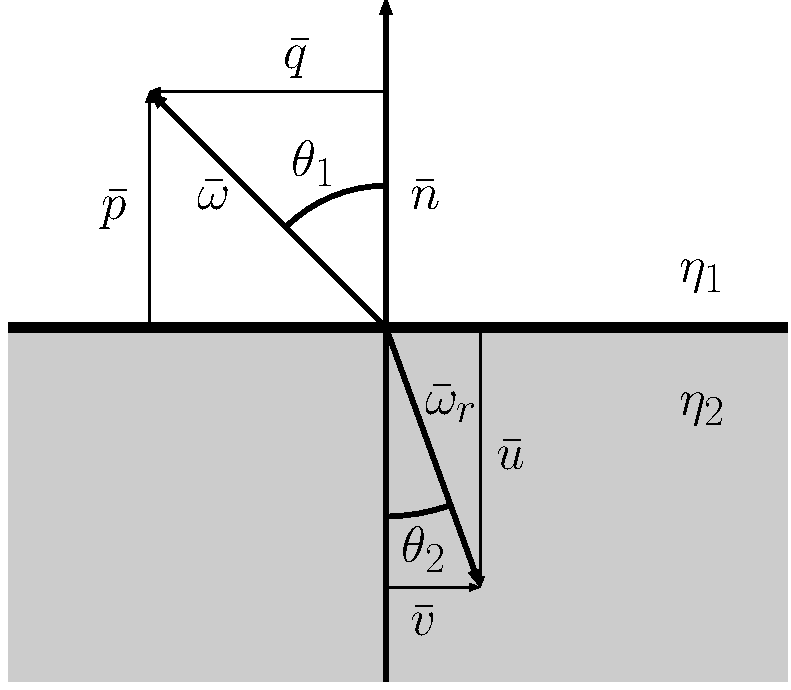
\includegraphics[width=0.8\textwidth]{drawing.pdf}
  \caption{Refrakcia lúča. (Pomocný obrázok k dôkazu)}
\end{figure}

\end{document}
